\documentclass[senior]{IPSstyle}

  \Year{2018}
  \Month{September}
  \Author{44161580-4: JIN YUTING}

  \Title{Flight schedule recovery with ant colony optimization}

  \Advisor{Professor Shigeru Fujimura}

\usepackage{amssymb,amsmath}

\usepackage{mathptmx}
\usepackage{helvet}
\usepackage{courier}
\usepackage{type1cm}

\usepackage{makeidx}
\usepackage{graphicx,subfigure}
\usepackage{multicol}
\usepackage{multirow}
\usepackage[bottom]{footmisc}

\usepackage{mathrsfs}
\usepackage{amssymb,amsmath}
\usepackage{amsfonts}
\usepackage{color}
\usepackage{CJKutf8}

\usepackage{listings}
\usepackage{algorithm,algorithmicx,algpseudocode}
\usepackage[toc,page,title,titletoc,header]{appendix}

\renewcommand{\algorithmicrequire}{\textbf{Input:}}
\renewcommand{\algorithmicensure}{\textbf{Output:}}

  \Abstract{
With the rapid development of air transportation demand, the contradiction between air traffic flow and capacity in airport terminal becomes more obvious. My research is to improve the rationality and effectiveness of flight recovery decision for unforeseen disruption, such as airport closure, and reduce the economic loss as much as possible. The goal is to aim to find feasible solution when flight disruption occurs using ant colony optimization method. The model include situation of flight cancellation and delay, fleet coordination. And we consider passenger satisfaction as an important factor. Test shows that the model in my research proved better randomness.
}

\Keywords{Airline Disruption Management,  Ant colony optimization}

\Acknowledgments{

Firstly, I would express my sincere thanks to Professor Fujimura. Professor Fujimura is a very affable supervisor, and gave me a lot of guidance and advice. I am truly thanks for his help.

I would also appreciate the IPS. Here is a suitable place for study. And I leave a lot of pleasant memory here.

Thanks my parents for their support and thanks all my friends who helped me study and minds.

Thank you all!



}


\begin{document}

 \makepreliminarypages
 \singlespace
 \frontmatter
 \tableofcontents
 \listoffigures
 \listoftables
 \mainmatter
 \clearemptydoublepage
 \setlength{\baselineskip}{23.0pt}

\chapter{Introduction} \label{introduction}



\section{Background}

\subsection{Current status of Chinese Aviation Industry}
In recent years, as an efficient transportation tool, airplane becomes a more and more common choice for travelling people. Statistics shows that in 2017 the number of passengers traveling by airplane is up to 4100 million worldwide. 
Since 1980s, Chinese civil aviation industry has been developing dramatically. 
From 2017 Civil Aviation Industry Development Statistics Bulletin\cite{timmurphy.org}, the total transport turnover volume was 1083.08 billion ton-kilometers, up 12.6\%, passenger transport volume was 9513.04 billion person-kilometers, up 13.5\%, and postal delivery volume was 243.55 billion ton-kilometers, up 9.8\%, compared with the data in 2016. 
In the past five years, the major transport indicator of Civil Aviation Administration of Chinese all increased with a dramatic speed, much higher than other transportation modes and average China's GDP growth level.

However, the rapid development of the civil aviation industry has also led to the increasingly serious flight delays.
Compared with developed country, Chinese civil aviation has higher flight delay frequency, longer delay time, more disputes between airline companies and passengers.
In the first two quarters of 2017, the average flight punctuality rate of Chinese Civil Aviation was 66.22\%, slipped 9.27\% year-on-year, with an average delay of 30 minutes, increased 11 minutes compared with the same period last year. With the influence of summer weather, the alignment rate dropped to 50\%.
Meanwhile, the total number of complaints received in 2017 increased by 29.3\% over the same period last year.
Therefore, flight delay problem of Chinese civil aviation has become an industrial public problem, which has led to a broad and sustained attention of the whole society.

In such circumstances, for Civil Aviation Administration Department of China and aviation transport enterprise, it has becomes an urgent problem to consider that how to control flight delay, improve flight punctuality rate and resolve disputes between passengers and airline companies caused by flight delays.

\subsection{Causes of flight delay}
In daily operation of airline company, flight delays are happening almost everyday.
According to the regulations on the normal statistics of civil aviation flights, flight delays are defined as:
\begin{itemize}
    \item flights that still did not take off in 15 minutes after the departure time published in timetable.
    \item flights that did not open the hatch at the arrival time published in timetable.
\end{itemize}
For this common phenomenon, there are some mean reasons. 

Weather factors, which cause the most frequent flight delays, should be considered first. 
Bad weather such as thunder, rain, fog and so on is force majeure events which is unpredictable and unavoidable. 
However in actual operation, fine weather at departure airport doesn't mean flights can take off successfully. 
Weather factors are usually analyzed at three points.
\begin{enumerate}
\item Whether the weather condition of departure airport is suitable for take-off. 
\item Whether the weather condition of destination airport is suitable for landing.
\item Whether the weather condition during the flight route is suitable for flying.
\end{enumerate}

In addition, even for same aircraft type, different airlines has great differences in specific safety standards.
And whether the flight will take off is also dependent on captain's judgment. 
The captain's decision on the current aircraft condition, airport and weather is also quite different.

The second leading reason is air traffic control. 
Due to recently explosive growth of air traffic flow, it is difficult for current flight management system to adapt. 
On the one hand, the development of corresponding ground facilities, equipment and service assurance can not keep up with high growth speed of civil aviation industry; 
on the other hand, current air route structure is no longer reasonable for increased air flow. 
So it has to be strictly restricted to the airspace.
And Air Force Activities may also lead to sudden air traffic control. In this case, passenger can only wait, no time to predict.

The third reason is aircraft failure.
Although most of hidden troubles can be dealt with in routine inspection, there is no guarantee that the aircraft equipment won’t suddenly fail. 
In order to ensure safety and completely eliminate hidden dangers, it always causes some delay. 
And if the airport that aircraft failure occurs is not airline’s aircraft maintenance base, the delay time will be so long and can’t be determined, even causes flight cancellations. 

The final reason is about passengers. 
Among all the reasons contributing to flight delay, the human factor of passenger's cause has become a "new growth point".
In order to wait or look around for a few passengers who are late, lost or does not heard of announcement, may also cause flight delays.
And sometimes a few minutes of delay may meet with longer delays caused by weather or air control.

Flight delays caused by reasons above is all dependent delay. In real life, we probably meet the delay caused by preceding flight delay. 
Usually, airlines plan flight schedule ahead of time, and to make profit maximization, they set flight schedule as intensive as possible. 
However, the shortage is that reduces robustness of whole airline network. With high density scheduling, once accidents occur, coordination becomes difficult.
Any omissions in the preceding flight may trigger a chain reaction of the subsequent flights. and the later flight is, the longer its delay time will be.
This kind of delay is going to be a more and more serious problem that forces airlines to confront.

%%%%%%%%%%%%%%%%%%%%%%%%%%%%%%%%%%%%%%%%%%%%%%%%%%%%%%%%%%%%%%%%%%%%%%%%%%%%%%%


\section{Motivation}
The operating goals of airline companies are reducing costs and improving profits as much as possible.
But accidents may disrupt original flight schedule, and cause economic losses to airline companies.
For airline, this loss can be divided into direct and indirect part.

Direct economic losses include loss of flight delay in ground-holding, loss of delay caused by air traffic jam, cost of accommodation for stranded passengers caused by long time delay or flight cancellation, and cost of temporary aircraft deployment. These extra costs directly increase airline company’s operation cost. 

In addition, flight delays also affect airline’s normal profit, cause indirect loss to airline company.

And for passengers, flight delay is also unpleasant experience. Flight delays or cancellation waste passenger’s private time and disrupt travel plans.

Besides huge economic losses for the airlines, flight disruption also bring great challenges to the normal operation of airports. Large scale of flight delays would disrupt airport running scheduling and cause a series of chain reactions. 

Therefore, when flight schedule was disrupted, how to make rescheduling in a short time has become an urgent need for the civil aviation industry. Rescheduling means to make a new schedule of affected flights based on original timetable.  The target is not only schedule the delayed flights with the best scheme, but also use as less time as possible. The rapider the recovery could be, the more the flight delay accumulation and the economic loss can be reduced.

%%%%%%%%%%%%%%%%%%%%%%%%%%%%%%%%%%%%%%%%%%%%%%%%%%%%%%%%%%%%%%%%%%%%%%%%%%%%%%%

\section{Organization of the thesis}
The rest of this thesis is structured as follows: Chapter 2 introduces some related works of past research in flight disruption management area. Chapter 3 introduces the application of ant colony optimization which is the main method of solving flight rescheduling problem, including the novelty of my research. In Chapter 4 I will explain implementation of ant colony optimization including evaluation process. Chapter 5 shows experiment using real world data and explains the conclusion. The last part, Chapter 6 describes the future works of this research.

%%%%%%%%%%%%%%%%%%%%%%%%%%%%%%%%%%%%%%%%%%%%%%%%%%%%%%%%%%%%%%Chapter 3
\chapter{Related Work} \label{related_work}

Flight schedule and recovery problem is a very practical problem and become more and more important nowadays. This is a typical scheduling problem. In the past research, there were two main research methods in this area, operation research and meta-heuristic. Clausen\cite{clausen2010disruption} made a through review of existing concept in airline disruption management area.

Teodorovic's\cite{teodorovic1984optimal} work aimed to find a new and more cohesive solution when some aircraft becomes unavailable and integrate crew and passengers at the same time. In 1993, Jarrah made some breakthrough. He chose network flow model, reducing the cost between 20\% to 90\%, compared with the solution not optimized. His test object is united airline's real flight. 

Thengvall\cite{thengvall2001multiple} applied integer programming into airline recovery problem. He used Continental Airline's real data to test his model, the result showed that his improvement was effective. But he only consider flight delay and flight cancellation in his model.
Wu and Gao\cite{wu2017rapid} also used integer programming method, combined with distributed network and his research was focused on the airport closure problem.

For research using meta-heuristic methods, Liu used Genetic Algorithm in his model and he applied Multi-Objective method to improve the evaluation process. But his test only took care of 70 flights and 7 aircraft which was too small and limited his study.

Zegordi and Jafari\cite{zegordi2010solving} used ant colony optimization method. Their model consider the real world constraints and real airline company regulations. The test showed that his approach can generate a feasible schedule in 5 seconds. Sousa\cite{sousa2015airline} also applied ant colony optimization method and proved his model better than depth-first search and breadth-first search. 

Castro\cite{castro2011new} used multi-agent system method to generate a new approach in airline disruption recovery management area. The innovation of this model was that he considered to avoid disruption and improve robustness of airline system by improving the pre-plan. Chiraphadhanakul\cite{chiraphadhanakul2013robust} also took the similar idea that re-allocation slack into original flight schedule so that could absorb more uncertainty.

All these research have improved the classical operational research methods. However, we believe that there will be a more cohesive solution, with higher effectiveness practicability in the future.
%%%%%%%%%%%%%%%%%%%%%%%%%%%%%%%%%%%%%%%%%%%%%%%%%%%%%%%%%%%%%%Chapter 4

\chapter{Methodology} \label{methodology}

\section{Data preprocess}

In this research, we get a dataset of original flight schedule from airline company at beginning.
This dataset includes flight id over a period of time, with its corresponding departure time and airport, landing time and airport, aircraft id and passenger information.
We consider a typical disruption like airport closure. 
It usually occurs unpredictably, and once it occurs, the closed airport will limit either departure or landing activities.
So when the bad weather causes airport closure, we suppose that airline company has internal notice of closure before real closure time for captains to react and we assume notice time is one hour earlier than closure time.
For optimization process, we intercept the flights from notice time to the end of that day.
Cause flight schedule is disrupted by one airport closure, we develop some rules for data preprocess before optimization process.
\begin{enumerate}
    \item Flights limitation: airport closure limits aircraft departure, so the flights which departure from closure airport with departure time after closure time will be cancelled.
    \item Aircraft availability: at the notice time, some aircraft have already been in mid-flight. For these aircraft, they will be available again after finishing current flight. The available time of these aircraft will be the landing time of their current flight, in the airport of their current flights’ landing airport.
    
    But there is a special series of aircraft should be considered. These aircraft departure before notice time so their captain will receive notice of airport closure during mid-flight. However, because these flights are scheduled to land at closed airport after closure time, they have to fly back to departure airport, and these aircraft can be used again at 
    \begin{equation*}
    notice\_time+(notice\_time-departure\_time.)    
    \end{equation*}
\end{enumerate}

With this preprocess above, we can get a list of flights remained and a series of aircraft available, and then generate flights information dataset and aircraft status dataset. With these two dataset, we can get the relationship between aircraft and flights and then calculate the feasible path matrix which will be used for following process. The specific step of preprocessing data will be explained in Chapter 4.

\section{Adjustment and evaluation}

\subsection{Flight adjustment method}
When a scheduled flight timetable is disrupted, for example, the bad weather causes airport closure or aircraft failure happens, we need to adjust the following flights. In general, there are some typical methods for adjustment.
\begin{enumerate}
    \item Adjust following flights’ departure time. This method can be considered as we allow delay in adjustment. Sometimes, delay is unavoidable, but we can make it as less as possible.
    \item Cancel the flight. In some circumstance, cancelling a flight and arranging redeeming flight on the next day will be better than delay for a long time. This is a method to make more reasonable use of aircraft resource.
    \item Change original aircraft-flight set. This means we assign a flight to an aircraft which different from the one on original schedule. Cause some aircraft may be spare and can be arranged for extra flights, this measure can utilize aircraft resource more effective.
    \item aircraft from other airports. In actual, this is not a common approach. Transferring means the aircraft need to take a flight with no passenger, so this method is only used when the disrupted flight is so important that cannot be cancelled. 
\end{enumerate}
%%%%%%%%%%%%%%%%%%%%%%%%%%%%%%%%%%%%%%%%%%%%%%%%%%%%%%%%%%%%%%%%%%%%%%%%%%%%%%%

\subsection{Objective Function}\label{section:Objective function}
In this research, we use total cost to evaluate each feasible solution. When a new feasible timetable be scheduled, the total cost can be calculated as below.
\begin{equation}\label{func:total cost}
    Total\ cost=C_a+C_d+C_c+C_p
\end{equation}
\begin{equation}\label{func:change aircraft cost}
    C_a = \sum_{f\in F} x_{f}*P_1
\end{equation}
\begin{equation}\label{func:delay cost}
    C_d =\sum_{f\in F} T_{d_f}*P_2
\end{equation}
\begin{equation}\label{func:cancel cost}
    C_c=\sum_{f\in F} z_{f}*P_3
\end{equation}
\begin{equation}\label{func:passsenger cost}
    C_p=\sum_{f\in F} y_f*T_{d_f}*NP_f*P_4+\sum_{f\in F} z_f*NP_f*P_5+\sum_{f\in F} (y_f+z_f)*CP_f*P_5
\end{equation}

\begin{table}
\renewcommand{\arraystretch}{1.0}
\label{piriform_dataset}
\begin{center}
\begin{tabular}{|c|c|}
\hline
\multicolumn{1}{|c|}{Var}
&\multicolumn{1}{c|}{Meaning}
\\
\hline
\(A\)	&	Set of all aircraft \(a\)
\\	\hline
\(F\)	&	Set of all flights \(f\)
\\	\hline
\(C_a\) &   Cost of changing aircraft.
\\  \hline
\(C_d\) &   Cost of delay.
\\  \hline
\(C_c\) &   Cost of cancellation.
\\  \hline
\(C_p\) &   Cost of passenger satisfaction.
\\  \hline
\(x_f\)	&   \(=0\), if flight\(f\) assigned to the same aircraft as original schedule; \(=1\), if not.
\\	\hline
\(y_f\) &   \(=1\), if flight\(f\) is delayed; \(=0\), if not.
\\  \hline
\(z_f\) &   \(=1\), if flight\(f\) is cancelled; \(=0\), if not.
\\  \hline
\(T_df\) &   The total delay time of flight\(f\) (minutes).
\\  \hline
\(NP_f\) &  Total number of passengers on flight\(f\).
\\  \hline
\(CP_f\) &   Number of passengers following with connecting flight on flight\(f\)
\\  \hline
\(P_1\) &   Cost of changing original aircraft for one flight.
\\  \hline
\(P_2\) &   Cost of delay for one flight per minute.
\\  \hline
\(P_3\) &   Cost of cancelling one flight.
\\  \hline
\(P_4\) &   Cost of maintaining passenger satisfaction for delaying flight per minute per passenger.
\\  \hline
\(P_5\) &   Cost of  maintaining passenger satisfaction for cancelled flight per passenger.
\\  \hline
\end{tabular}
\caption{Parameters and Variables}
\end{center}
\end{table}

Based on the one in \cite{sousa2015airline}, the model in this research made some change. Corresponding to different adjustment method, the total cost is divided into four parts Fig.\ref{fig:coststructure}: cost of changing aircraft, cost of delay, cost of cancellation and cost of passenger satisfaction maintenance. Evaluation is in airline company’s view, so the passengers’ satisfaction can be quantified as a kind of cost. And in this part, we consider a special class of passengers with connecting flights. These passengers purchase more than one tickets at one-time and need to take a transit in midway. So it will do great effect on the rest of their journey if the first flight in connecting flights is delayed. There will also be probably for them to miss the next flight. 

To calculate the cost of part, we need to know the status of each flight in new feasible solution. 
In this research, there are three indicators to represent the three flight status: changed aircraft, delayed and cancelled. 

\begin{figure}[h]
    \centering
    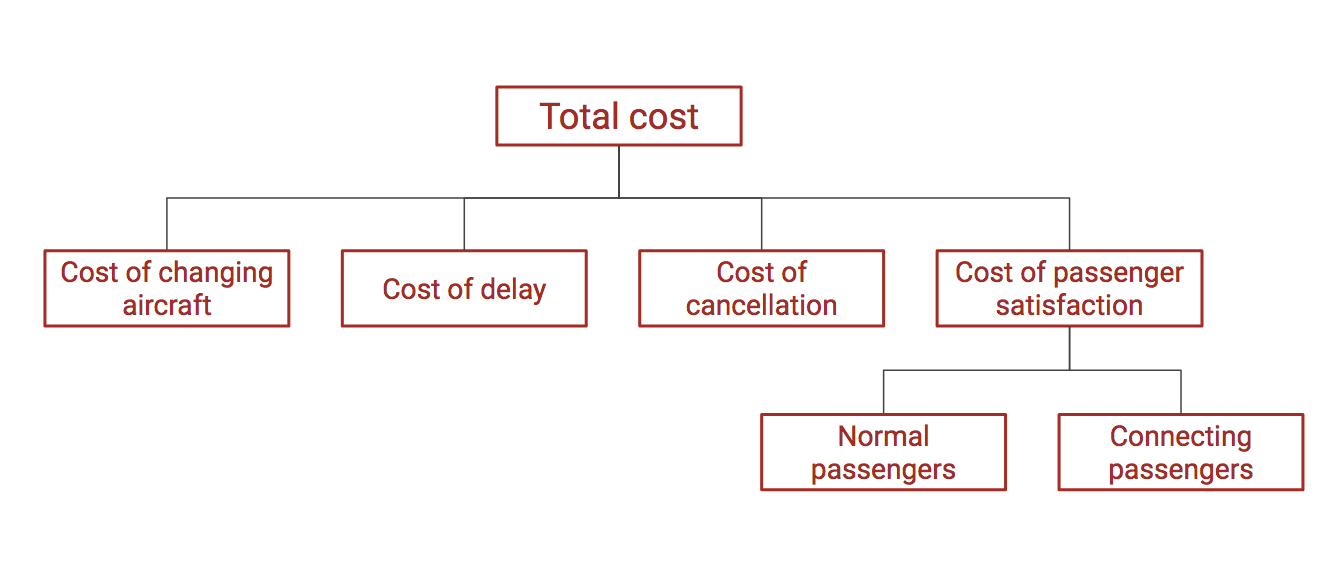
\includegraphics[width=15cm]{MasterThesis-master/Coststructure.png}\\
    \caption{Structure of total cost}
    \label{fig:coststructure}
\end{figure}

\(x_f\) indicates the status that if the flight \(f\)is assigned to the same aircraft as original schedule. \(y_y\) indicates the status that if the flight \(f\) is delayed. And \(z_f\) indicates the status that if the flight \(f\) is cancelled. \(x_f\), \(y_f\) and \(z_f\) is Boolean value(0 or 1).
%%%%%%%%%%%%%%%%%%%%%%%%%%%%%%%%%%%%%%%%%%%%%%%%%%%%%%%%%%%%%%%%%%%%%%%%%%%%%%%
\section{Ant colony optimization} \label{Ant colony optimization}

In my research, I apply ant colony optimization for flight rescheduling problem. And in evaluation part, I use cost to measure feasible solutions of each iteration. I build the model based on past thesis\cite{sousa2015airline} and enlarge the scope of the problem. I will explain specifically below. 

\begin{figure}[h]
  \centering
  % Requires \usepackage{graphicx}
  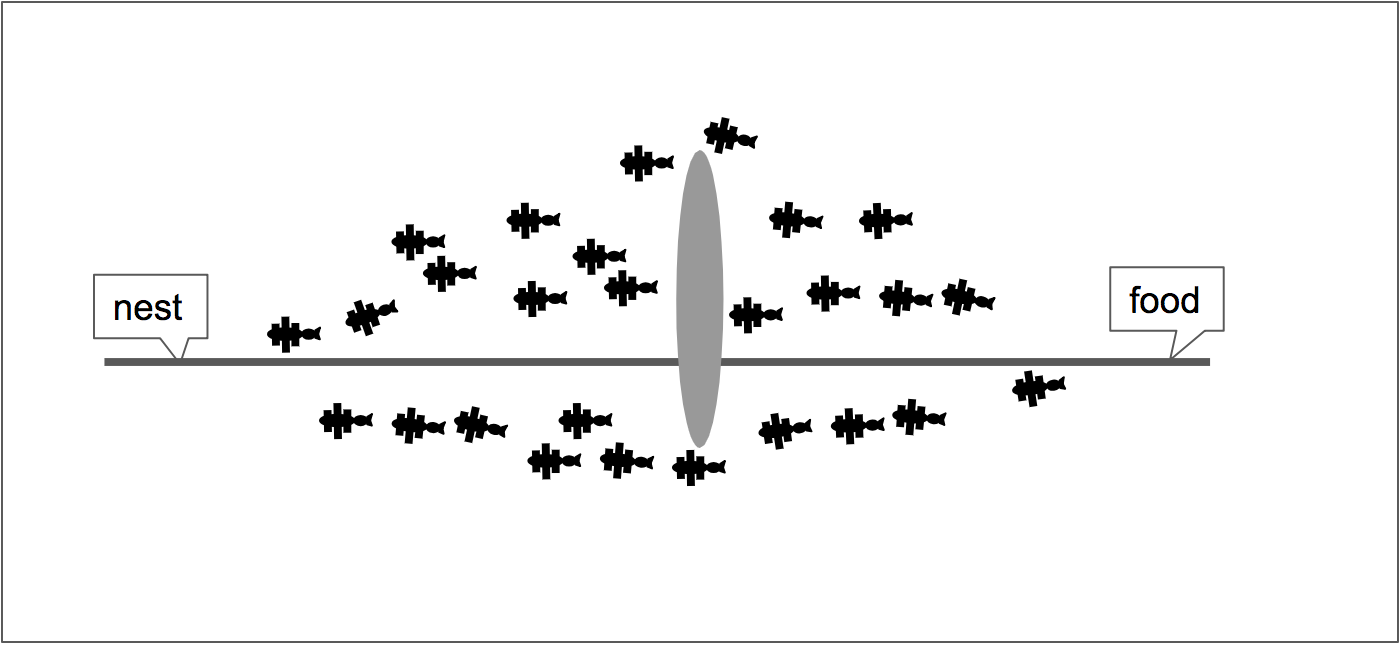
\includegraphics[width=15cm]{MasterThesis-master/ACO-1.png}\\
  \caption{At beginning ants choose paths randomly.}\label{fig: aco1}
\end{figure}

\begin{figure}[h]
    \centering
    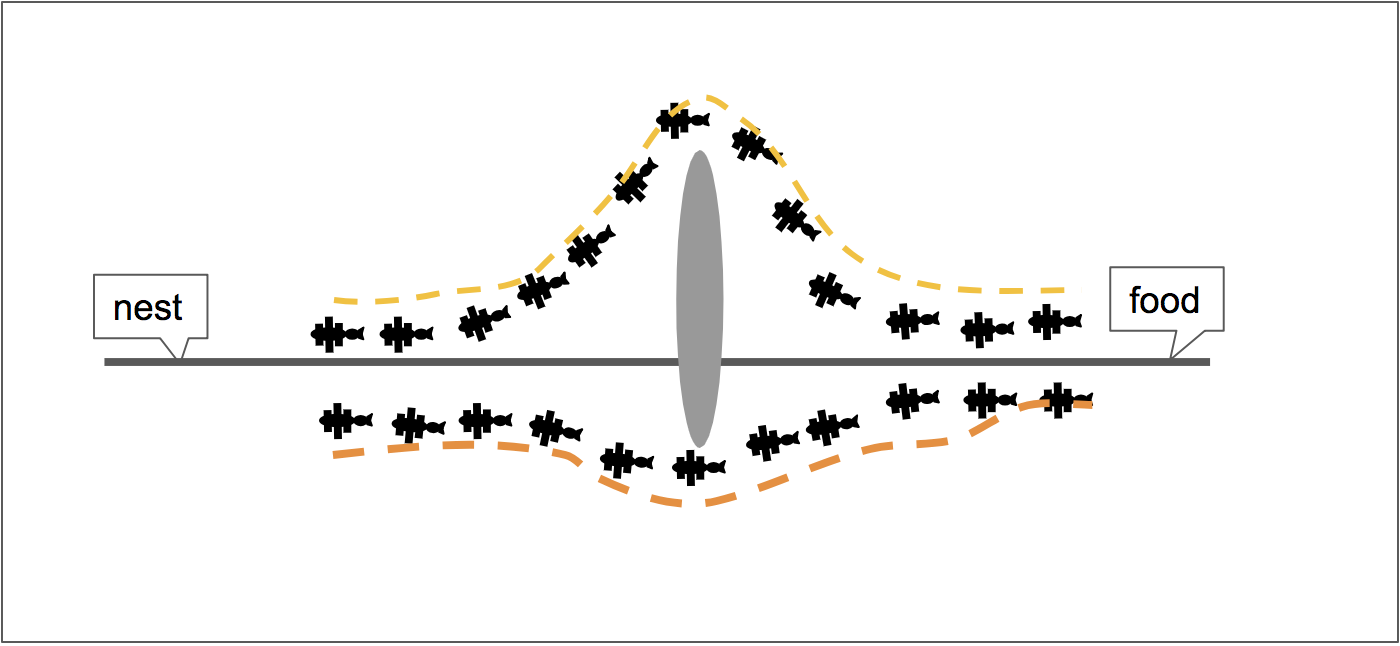
\includegraphics[width=15cm]{MasterThesis-master/ACO-2.png}
    \caption{Ants leaves pheromone on the paths passed.}
    \label{fig:my_label1}
\end{figure}

\begin{figure}[h]
    \centering
    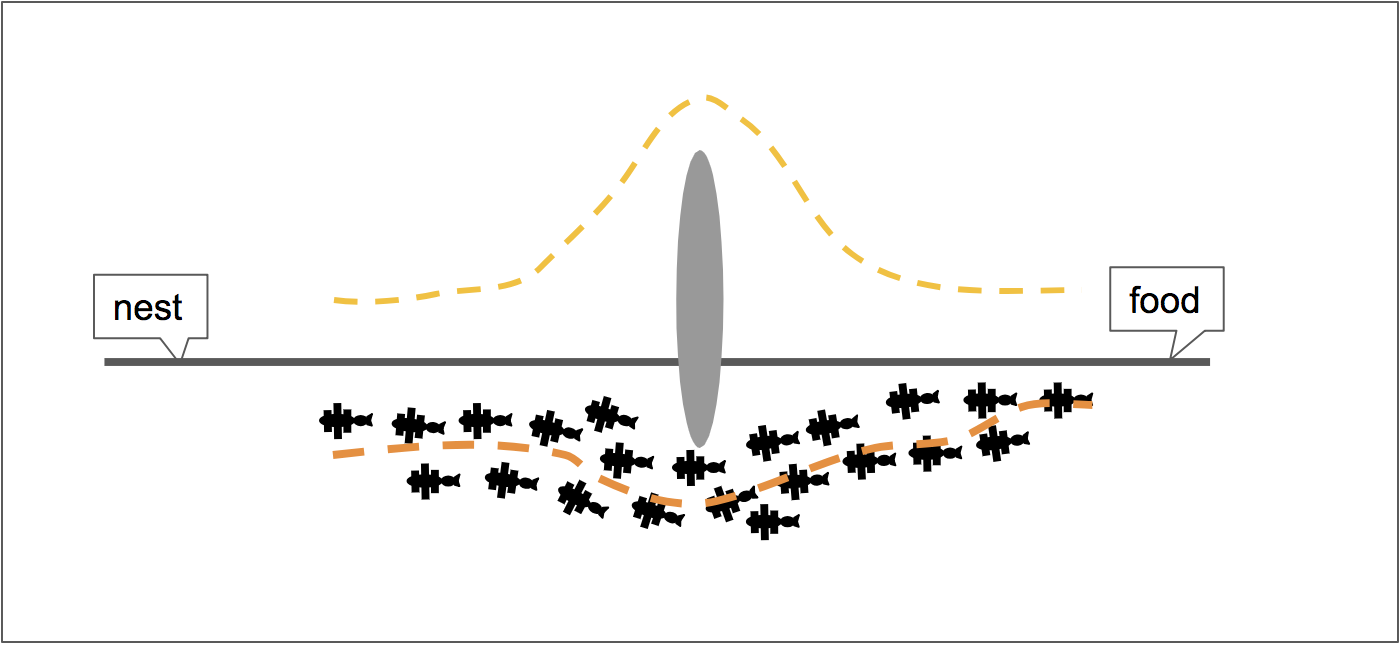
\includegraphics[width=15cm]{MasterThesis-master/ACO-3.png}
    \caption{Finally ants will find optimum route with higher pheromone concentration.}
    \label{fig:my_label2}
\end{figure}

As a meta-heuristic algorithm, ant colony optimization is an optimization algorithm simulating foraging behavior of ants. The basic principle of ant colony algorithm is:
\begin{enumerate}
    \item During foraging process, ants release pheromones on the passed path.
    \item When an ant meets an intersection that has not yet passed, it will pick one direction randomly. At the same time, the ant releases pheromones on the path.
    \item When ants later meet the intersection, they will the path with a higher concentration of pheromone.
    \item The concentration of pheromone is related to the length of path and is inversely proportional to it. The shorter the path is, the higher the concentration can be.
    \item When the number of ant increases, the pheromone concentration on the optimal path is increased.
    \item As time goes on, the whole ant colony finally find the optimal foraging route.
\end{enumerate}

Ant colony algorithm  was used to solve traveling salesman problem(TSP) at beginning. 
So in my model, I try to use a whole path to represent a feasible schedule solution. 
Considering both flights and aircraft as cities in TSP, the path between each two cities indicates the relationship between flights and flights or aircraft and flights. 
And in flight schedule problem, the final goal is minimum the whole cost. So when we get a feasible route, we can calculate the total cost and consider it as the distance in TSP.

In this algorithm, for each iteration, we have more than one ants and every ant can be seen as a simple agent. There are some constraints:
\begin{enumerate}
    \item One iteration only allows each ant move one step;
    \item For each step, each ant leaves pheromones on the branches that they pass through;
    \item The probability for ants to choose next node is related to the pheromone concentration contained in the linked branch;
    \item Use tabu list to represent nodes that have been passed.
\end{enumerate}

For basic ant colony algorithm, there are two main process:
\begin{enumerate}
    \item State Transition:
    
    In each iteration, every ant moves one step, the probability of ant \(k\) to move from state \(i\) to state \(j\),can be calculated by this function:
    \begin{eqnarray}\label{probability}
    p_{ij}^k &=&
    \begin{cases}
    \cfrac{[\tau(i,j)]^\alpha [\eta(i,j)]^\beta}{\sum_{z\in J_k(i)} [\tau(i,z)]^\alpha [\eta(i,z)]^\beta} &, j\in allowed_k \cr
    0 \cr
    \end{cases}
    \end{eqnarray}
    In this function, \(\tau(i,j)\) means the pheromone concentration on the branch between node \(i\) and \(j\), \(\eta(i,j)\) represents the desirability of transforming states.(In TSP it is \(1/distance\), but in this research it is \(1/cost\)). 
    
    \(\alpha\) is heuristic factor, controls influence of residual pheromone concentration. The larger the \(\alpha\) is, the greater the possibility of ants choosing the path they have passed before can be, and The randomness of search will be weakened. \(\beta\) is expectation heuristic factor. When \(\beta\) increased, the convergence speed also increased, and the algorithm is more likely to fall in local optimum. 
    Usually, the range of \(\alpha\) is \([0,5]\), and the range of \(\beta\) is  \([0,5]\).
    
    In past thesis\cite{sousa2015airline}, ant chooses the next node only depends on the pheromone concentration on the path that connecting that node and the current one. But this causes a problem that the path ants passed will have higher pheromone concentration and ants would more likely to choose the path that passed before, so the model will rapidly fall into local optimum.
    
    So we make some improvement of the selecting next node process. After calculating the probability of each path, we made each probability to minus a random number. That may cause some probability less than 0. And then we choose the path with highest probability. Because the number that each probability minus is random and different from one to another, so it can randomly disorder the sequence of probability and add randomness into the whole system. This approach helps model not fall in local optimum too fast.
    
    \item Pheromone Update
    
    For process of updating pheromone matrix, there have been three models.
    \begin{itemize}
        \item Ant-Cycle model:  The increment of pheromone is related to the whole route of search, not related to the specific path choice. This approach updates pheromone amount of all paths on the route after completing a complete path search. It is a global updating method.
        \item Ant-Quantity model: The increment of pheromone is related to the distance of specific path(i,j). This approach is a local updating method and updates pheromone amount on the path after each step of ants.
        \item Ant-Density model: The increment of pheromone is fixed and is also a local updating method.
    \end{itemize}
    In this research, cause the cost can only be calculated after we get a complete fleet schedule, I choose global updating method for each iteration.
    
    And at time \((t+n)\), the pheromone concentration on the path\((i,j)\) can be calculated as:
    \begin{equation}
        \tau _{ij}(t+n)=(1-\rho)\cdot \tau _{ij}(t)+\Delta\tau _{ij}(t)
    \end{equation}
    \begin{equation}
        \Delta\tau _{ij}(t) = 1/Total\ cost
    \end{equation}
    \(\rho\) represents the evaporation factor. If \(\rho\) is too small, the pheromone remained on each path will be too much, and influence the convergence speed; but if \(\rho\) is too big, some effective path will be skipped. 
    
    \(m\) is the total number of ant colony. The larger the \(m\) is, the  more accurate the result will be. But if the \(m\) is too big, it will slow down the speed of computing.
\end{enumerate}

 


\section{Enhanced Problem} \label{innovation}
In this model, we try to widen the scope of flight recovery problem with application of ant colony optimization. H. Sousa(2015)\cite{sousa2015airline} considered a disruption scenario of aircraft failure during a time period. In this research, we consider a more complicated circumstance of airport closure which is also more close to reality. When airport closure (usually caused by bad weather) happens, it will influence a series of flights and limit aircraft’s departure and landing. The challenge is this problem involves a large number of flights and status of flight and aircraft is changing over the time, that brings difficulty to optimization. So before optimization process, we do data preprocessing first. In this part we group these flights and aircraft according to their different status and handle them separately. That will make the problem clearer and easier for following optimization process.

Another improvement is that we divide passengers into two parts and consider those passengers buy connecting flights. In past research\cite{sousa2015airline}, maintaining passengers’ satisfaction is considered as an important influencing factor, but it is analyzed as a whole unit. In this research, we think passengers with connecting flights are special, because if the delayed or cancelled flight is their first flight of connecting tickets, they will suffer greater impacts than other passengers. So in this model, no matter the flight is delayed or cancelled, we assume that the passengers with connecting tickets on this flight cannot catch the next flight. So that delaying or cancelling flights with connecting passengers will have higher punishment and cost more.

For algorithm, we add randomness in selecting next node part. In each iteration, every ant creates its own route and it chooses the next node by probability. This probability is calculated by the pheromone value on the path connecting the current node and the next one. However, it we only use this rules, ants will more likely to choose the path that have been past before. So we insert some randomness into selecting process. In this way, ants will have more probability to choose path randomly in the first couple of iteration, and the algorithm can avoid falling into local minimum too fast.


%%%%%%%%%%%%%%%%%%%%%%%%%%%%%%%%%%%%%%%%%%%%%%%%%%%%%%%%%%%%%%%%%%%%%%%%%%%%%%%


\chapter{Proposed algorithm with Ant Colony Optimization} \label{implement}
In this section, I will explain the specific step of optimization process and use a couple of flights as an example. At the beginning of the whole process, the input is original flight schedule and disruption scenario includes the time and location of occurrence. And our goal is to output a feasible solution with fitness which is total cost in this model as less as possible using ant colony optimization.

\section{Preparation}

At the beginning, we get an original schedule dataset over a period of time, some days or one month. This dataset includes too much information so that will be difficult to use this dataset for following computing. So we create another two dataset based on this original one. The first is flight information dataset, which includes flights’ id, departure and landing time, departure and landing airport, the number of total passengers and passengers with connecting tickets, total flying time and original aircraft pair(aircraft pair means the aircraft that a flight planned to be assigned in original schedule). Second one is aircraft status dataset, which records the status of each aircraft at the process beginning moment, includes aircraft's id, available time, current location and available seats number.

\begin{table}[t]
\renewcommand{\arraystretch}{1}
\label{Flight_information_dataset}
\begin{center}
\begin{tabular}{|c|c|}
\hline
\multicolumn{1}{|c|}{Attribute}
&\multicolumn{1}{c|}{Meaning}
\\
\hline
\(flight\_id\)	&	Unique for each flight
\\	\hline
\(departure\_time\)	&	Original departure time
\\	\hline
\(departure\_airport\) &   departure airport, cannot be changed
\\  \hline
\(landing\_time\) &   Original landing time
\\  \hline
\(landing\_airport\) &   Flight's destination
\\  \hline
\(flying\_time\) &   Calculated by its departure time and landing time
\\  \hline
\(num\_passengers\)	&   Number of total passengers on flight
\\  \hline
\(num\_connecting\_passenger\) &   Number of passengers with following connecting flight
\\  \hline
\(aircraft\_id\) &   The original aircraft which flight is  assigned to
\\  \hline
\end{tabular}
\caption{Flight information}
\end{center}
\end{table}

\begin{table}
\renewcommand{\arraystretch}{1.2}
\begin{center}
\begin{tabular}{|c|c|}
\hline
\multicolumn{1}{|c|}{Attribute}
&\multicolumn{1}{c|}{Meaning}
\\  \hline
\(aircraft\_id\)	&	Unique for each aircraft
\\	\hline
\(available\_time\)	&	The time that aircraft can be firstly used(generally is the begin time of process
\\	\hline
\(current\_airport\) &  The location of aircraft at beginning
\\  \hline
\(num\_seats\) &  Accommodating number of this aircraft
\\  \hline
\end{tabular}
\caption{Aircraft status}
\label{Aircraft_status_dataset}
\end{center}
\end{table}

Then, we insert disruption scenario. Disruption is reflected as closed airport id and time of closure. To make it more like real life, we suppose a notice time which is the time that airline publish internal closure information to captains. We suppose the disruption happens so suddenly that the flights planned to departure before notice time are processed normally. And we use this notice time as the process start time. Using this disruption information, combined with original schedule,  we can get two dataset mentioned above based on the rules below.

Flight information: we only arrange flights in one day.
\begin{enumerate}
    \item intercept the flights which planned to departure after notice time and before the end of the day.
    \item the flights planned to departure after closure time from closed airport are cancelled and remove from dataset.
\end{enumerate}

Aircraft status: we consider notice time as a boundary. 
\begin{enumerate}
    \item If the aircraft is not in flight at the moment of notice time, the aircraft’s available time is notice time, and its current location is landing airport of its last flight. 
    \item For flight on mid-flight at notice time, there are two circumstance.
    \begin{itemize}
        \item If the aircraft originally scheduled to land on closed airport after closure time, this aircraft need to return its departure airport, so its current location is its current flight’s departure airport, and its available time is $notice\_time+ (notice\_time - departure\_time)$
        \item if aircraft’s current flight is not influenced by airport closure, this aircraft’s available time is the landing time of its current flight and current location is landing airport of its current flight.
    \end{itemize}
\end{enumerate}
These two dataset will be the basis of following process.

\section{Schedule Representation}\label{Section:relationship}

In this research, we use ant colony optimization as the main algorithm, so there is a key point that we should use a continuous path to represent one feasible schedule solution including both flights and aircraft. The difficult point is how to find feasible path at first. After preprocess, we have flight information dataset and aircraft status dataset. And I will use a small example to explain how to generate feasible paths. 

As shown in Table \ref{Example flight information} and \ref{Example aircraft status}, this example includes six flights and three aircraft.

\begin{table}[h]
\renewcommand{\arraystretch}{1.2}
\begin{center}
\begin{tabular}{|c|c|c|c|c|c|c|}
\hline
\multicolumn{1}{|c|}{flight\_id}
&\multicolumn{1}{c|}{\(F866\)}
&\multicolumn{1}{c|}{\(F874\)}
&\multicolumn{1}{c|}{\(F890\)}
&\multicolumn{1}{c|}{\(F904\)}
&\multicolumn{1}{c|}{\(F2304\)}
&\multicolumn{1}{c|}{\(F2307\)}
\\  \hline
departure\_time & 8:35 & 12:30 & 10:20 & 14:10 & 16:55 & 19:10
\\	\hline
landing\_time & 11:25 & 15:20 & 13:05 & 16:55 & 18:25 & 20:30
\\	\hline
departure\_airport & 49 & 46 & 49 & 46 & 46 & 45
\\  \hline
landing\_airport & 46 & 49 & 46 & 49 & 45 & 46
\\  \hline
flying\_time & 2:50 & 2:50 & 2:45 & 2:45 & 1:30 & 1:20
\\  \hline
aircraft\_id & 42 & 42 & 58 & 58 & 62 & 62
\\  \hline
num\_passengers & 86 & 117 & 114 & 132 & 131 & 107
\\  \hline
num\_connecting\_passenger & 0 & 0 & 0 & 0 & 16 & 58
\\  \hline
\end{tabular}
\caption{Example flight information}
\label{Example flight information}
\end{center}
\end{table}

\begin{table}[h]
\renewcommand{\arraystretch}{1}
\begin{center}
\begin{tabular}{|c|c|c|c|}
\hline
\multicolumn{1}{|c|}{aircraft\_id}
&\multicolumn{1}{c|}{available\_time}
&\multicolumn{1}{c|}{current\_airport}
&\multicolumn{1}{c|}{num\_seats}

\\  \hline
A42 & 8:35 & 49 & 119
\\	\hline
A62 & 8:35 & 46 & 161
\\	\hline
A42 & 8:35 & 49 & 161
\\  \hline
\end{tabular}
\caption{Example aircraft status}
\label{Example aircraft status}
\end{center}
\end{table}

\begin{figure}[h]
    \centering
    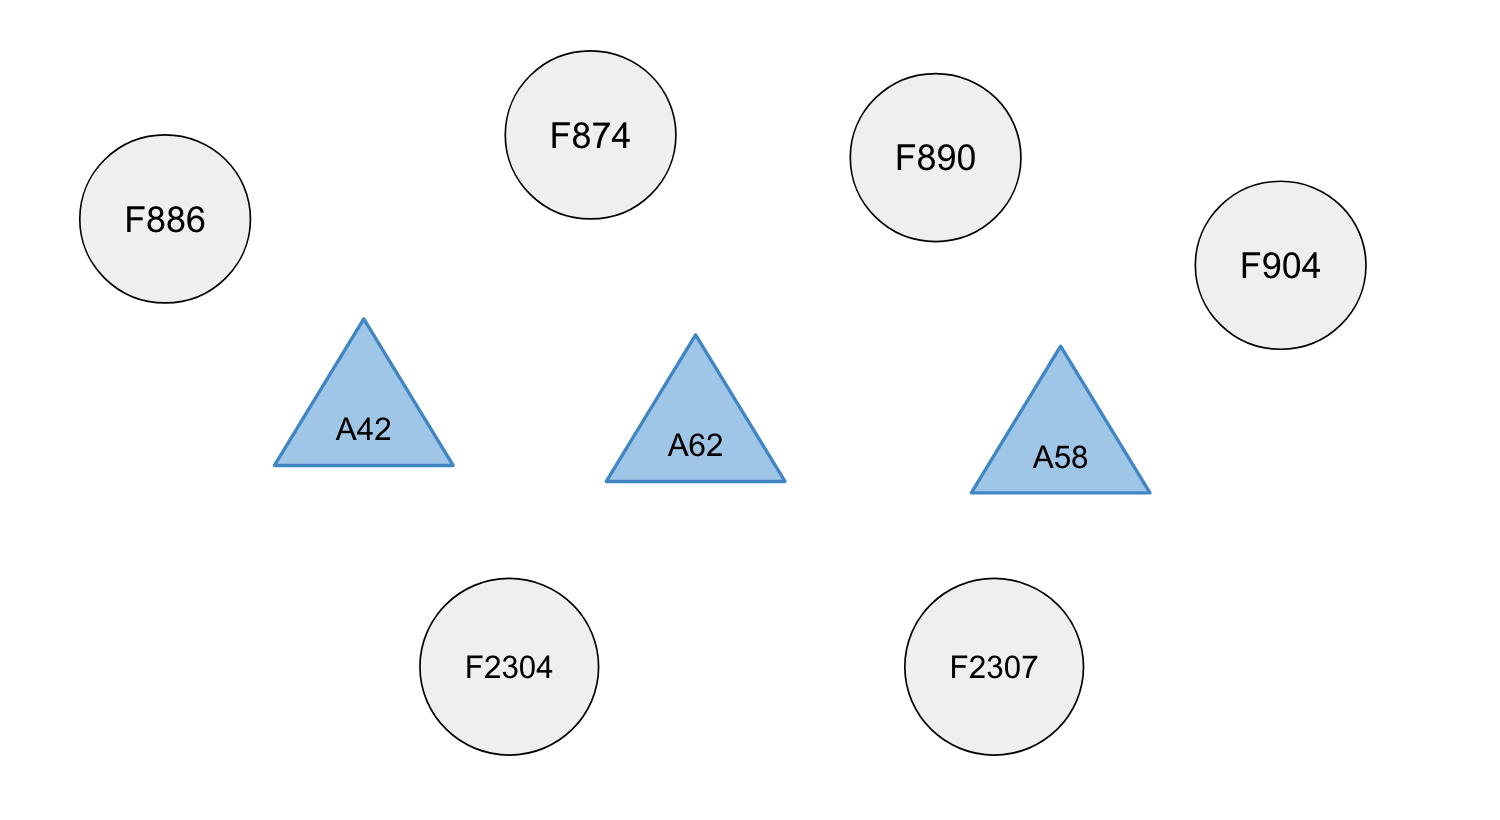
\includegraphics[width=15cm]{MasterThesis-master/nodes.png}\\
    \caption{Aircraft nodes and flight nodes}
    \label{fig:nodes}
\end{figure}
We use Fig.\ref{fig:nodes} to represents these flights and aircraft. The round nodes represent flights, and triangle nodes represent aircraft.

Firstly, we get the relationship between flights and flights. If the two flight \(f_1\) and \(f_2\) satisfy the following conditions, then there will be a feasible path from \(f_2\) to \(f_1\):
\begin{itemize}
    \item The departure airport of flight \(f_1\) is same as flight \(f_2\) 's landing airport.
    \item The departure time of flight \(f_1\) is later than the departure time of flight \(f_2\).
\end{itemize}
Then we can get feasible paths shown in Fig.\ref{fig:f2f}. And with this path web, we can use a feasible path table to represent this relationship. In Table.4.5, \(1\) means there is a feasible path from row to column and \(0\) means the path is not feasible. 
\begin{figure}[h]
    \centering
    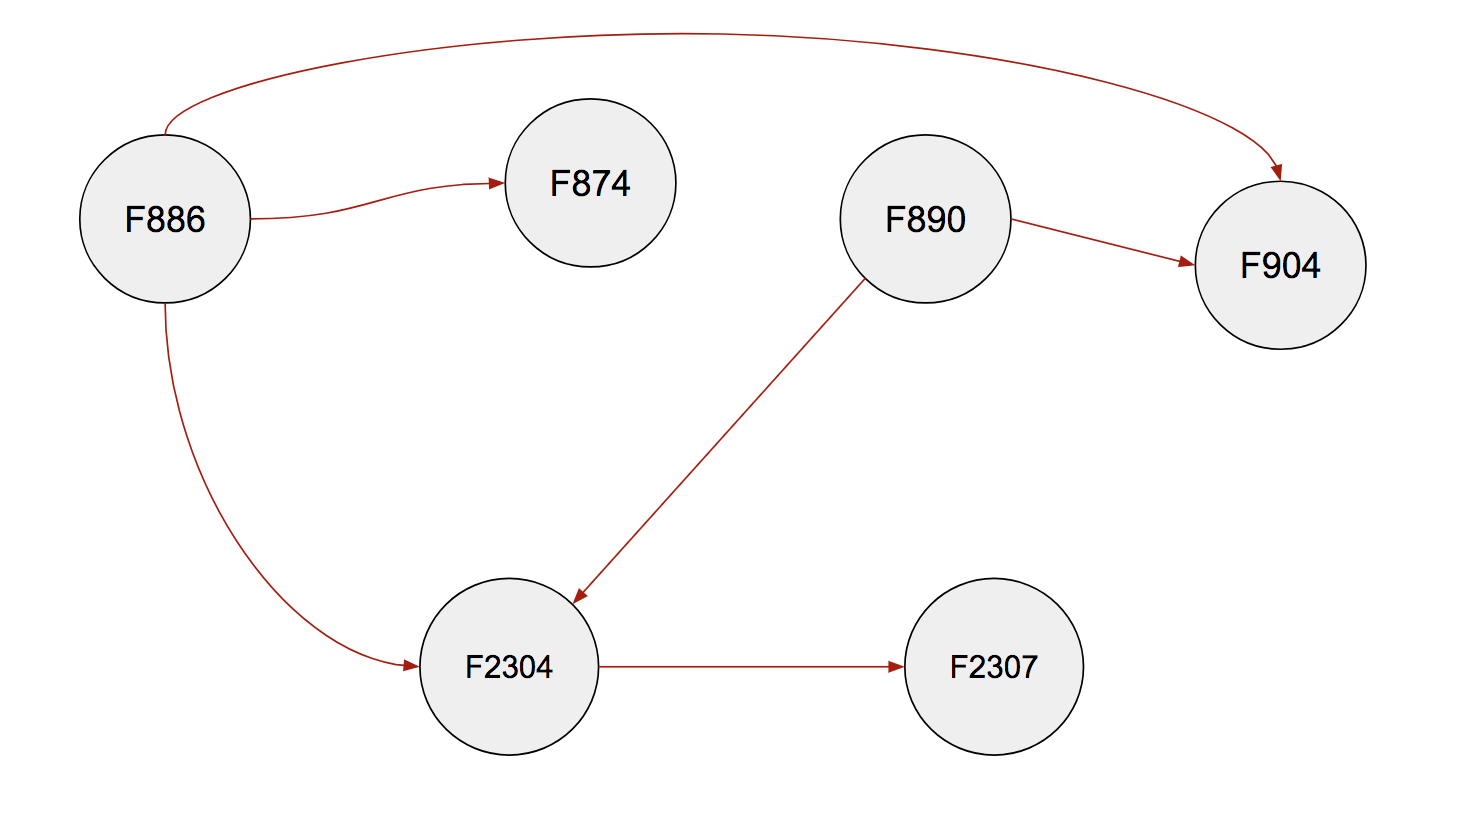
\includegraphics[width=15cm]{MasterThesis-master/f2f.png}\\
    \caption{Feasible paths between flight nodes}
    \label{fig:f2f}
\end{figure}

\begin{table}[h]
\renewcommand{\arraystretch}{1}
\label{table:f2f}
\begin{center}
\begin{tabular}{|c|c|c|c|c|c|c|}
\hline
\multicolumn{1}{|c|}{}
&\multicolumn{1}{|c|}{\(F866\)}
&\multicolumn{1}{c|}{\(F874\)}
&\multicolumn{1}{c|}{\(F890\)}
&\multicolumn{1}{c|}{\(F904\)}
&\multicolumn{1}{c|}{\(F2304\)}
&\multicolumn{1}{c|}{\(F2307\)}

\\  \hline
\(F866\) & 0 & 1 & 0 & 1 & 1 & 0
\\	\hline
\(F874\) & 0 & 0 & 0 & 0 & 0 & 0
\\	\hline
\(F890\) & 0 & 0 & 0 & 1 & 1 & 0
\\  \hline
\(F904\) & 0 & 0 & 0 & 0 & 0 & 0
\\  \hline
\(F2304\) & 0 & 0 & 0 & 0 & 0 & 1
\\  \hline
\(F2307\) & 0 & 0 & 0 & 0 & 0 & 0
\\  \hline
\end{tabular}
\caption{Feasible paths between flights and flights}
\end{center}
\end{table}

Secondly, we explore feasible path form aircraft to flights.
If aircraft \(a\) and flight \(f\) satisfy the following conditions, then there will be a feasible path from \(a\) to \(f\):
\begin{itemize}
    \item The current location of aircraft \(a\) is the same as flight \(f\) ’s departure airport;
    \item The departure time of flight\(f\) is later than the available time of aircraft \(a\);
    \item Aircraft \(a\) has required passenger seats of flight \(f\).
\end{itemize}
Using example data, the feasible paths from aircraft to flights can be represented by Fig.\ref{fig:a2f}. And we also use a 0-1 table Table \ref{Example Feasible paths a2f} to record this relationship.

\begin{figure}[h]
    \centering
    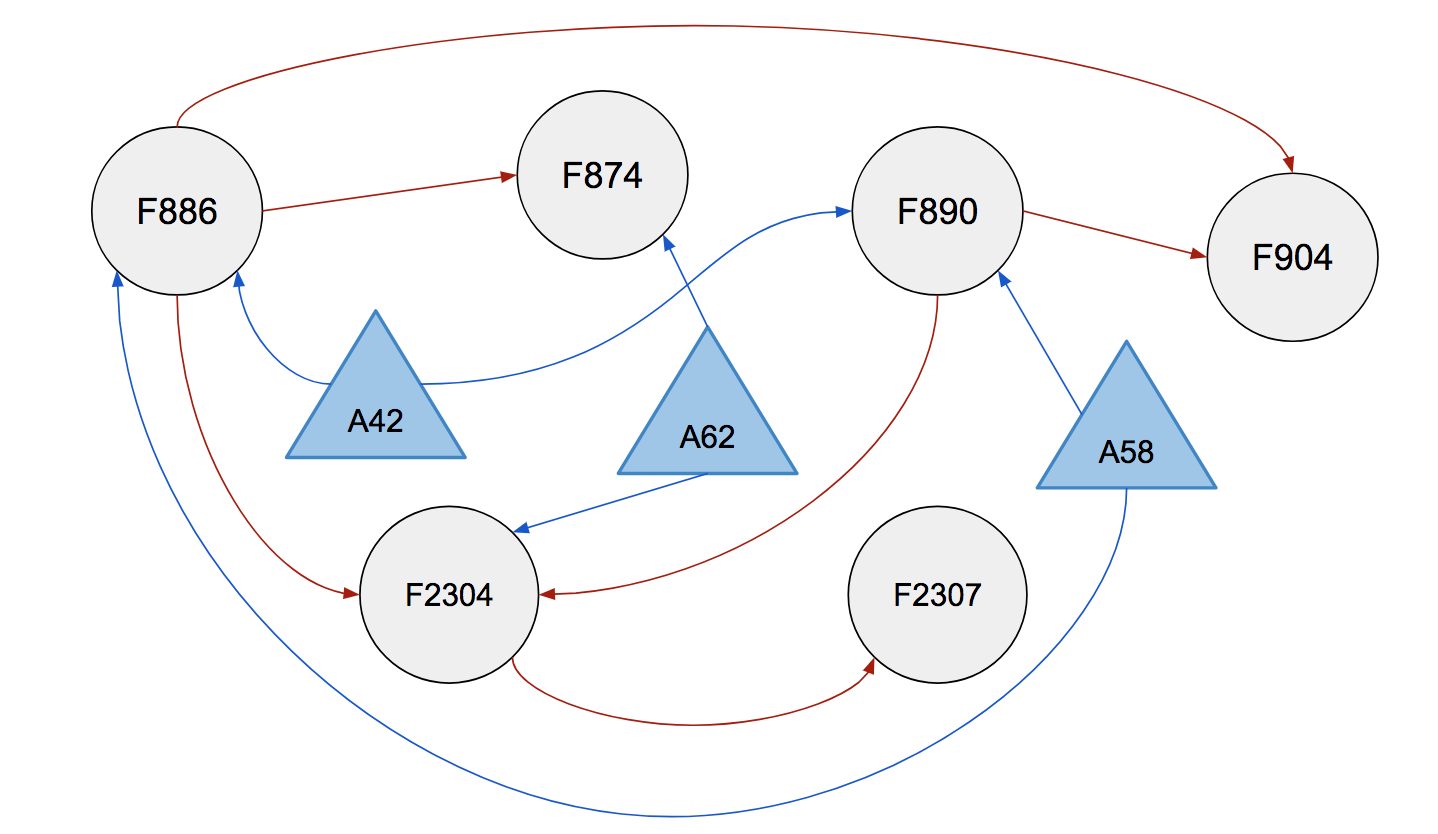
\includegraphics[width=15cm]{MasterThesis-master/a2f.png}\\
    \caption{Feasible path between aircraft nodes and flight nodes}
    \label{fig:a2f}
\end{figure}

\begin{table}[h]
\renewcommand{\arraystretch}{1}
\begin{center}
\begin{tabular}{|c|c|c|c|c|c|c|}
\hline
\multicolumn{1}{|c|}{}
&\multicolumn{1}{|c|}{\(F866\)}
&\multicolumn{1}{c|}{\(F874\)}
&\multicolumn{1}{c|}{\(F890\)}
&\multicolumn{1}{c|}{\(F904\)}
&\multicolumn{1}{c|}{\(F2304\)}
&\multicolumn{1}{c|}{\(F2307\)}
\\  \hline
\(A42\) & 1 & 0 & 1 & 0 & 0 & 0
\\	\hline
\(A58\) & 1 & 0 & 1 & 0 & 0 & 0
\\	\hline
\(A62\) & 0 & 1 & 0 & 0 & 1 & 0
\\  \hline
\end{tabular}
\caption{Feasible path between aircraft nodes and flight nodes}
\label{Example Feasible paths a2f}
\end{center}
\end{table}

And finally, in order to find one path that can go through all aircraft nodes, all the path should be linked together. So all the nodes(include aircraft and flights) has path to aircraft nodes in spite of their departure time or location. The Fig.\ref{fig:all feasible paths} shows the completed web of all feasible paths based on original schedule. 
We use Table\ref{a2a & f2a} to represent the relationship between all nodes to aircraft nodes. 

\begin{figure}[h]
    \centering
    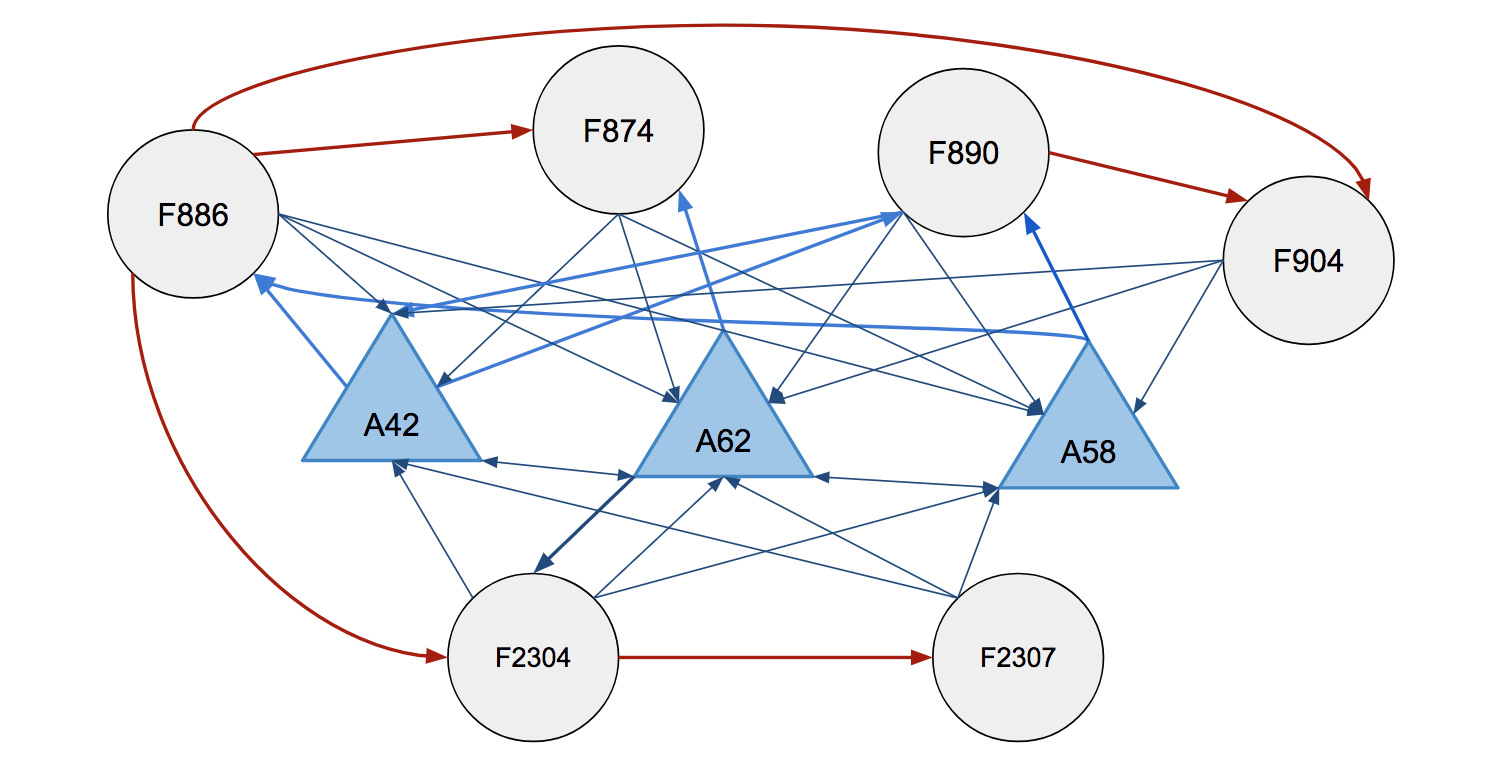
\includegraphics[width = 15cm]{MasterThesis-master/completed-web.png}\\
    \caption{All feasible paths}
    \label{fig:all feasible paths}
\end{figure}

\begin{table}[h]
\renewcommand{\arraystretch}{1}

\begin{center}
\begin{tabular}{|c|c|c|c|}
\hline
\multicolumn{1}{|c|}{}
&\multicolumn{1}{|c|}{\(A42\)}
&\multicolumn{1}{c|}{\(A58\)}
&\multicolumn{1}{c|}{\(A62\)}
\\  \hline
\(A42\) & 0 & 1 & 1
\\	\hline
\(A58\) & 1 & 0 & 1
\\	\hline
\(A62\) & 1 & 1 & 0 
\\  \hline
\(F866\) & 1 & 1 & 1
\\	\hline
\(F874\) & 1 & 1 & 1
\\	\hline
\(F890\) & 1 & 1 & 1
\\  \hline
\(F904\) & 1 & 1 & 1
\\  \hline
\(F2304\) & 1 & 1 & 1
\\  \hline
\(F2307\) & 1 & 1 & 1
\\  \hline
\end{tabular}
\caption{Feasible path to aircraft nodes}
\label{a2a & f2a}
\end{center}
\end{table}

And we merge Table\ref{fig:f2f},Table\ref{fig:a2f} and \ref{a2a & f2a}together to get Table\ref{all paths}.
This is the feasible paths between all nodes based on the original schedule. If there is any flight change happens, this table will be updated.

\begin{table}[h]
\renewcommand{\arraystretch}{1}
\begin{center}
\begin{tabular}{|c|c|c|c|c|c|c|c|c|c|}
\hline
\multicolumn{1}{|c|}{}
&\multicolumn{1}{|c|}{\(A42\)}
&\multicolumn{1}{c|}{\(A58\)}
&\multicolumn{1}{c|}{\(A62\)}
&\multicolumn{1}{|c|}{\(F866\)}
&\multicolumn{1}{c|}{\(F874\)}
&\multicolumn{1}{c|}{\(F890\)}
&\multicolumn{1}{c|}{\(F904\)}
&\multicolumn{1}{c|}{\(F2304\)}
&\multicolumn{1}{c|}{\(F2307\)}
\\  \hline
\(A42\) & 0 & 1 & 1 & 1 & 0 & 1 & 0 & 0 & 0
\\	\hline
\(A58\) & 1 & 0 & 1 & 1 & 0 & 1 & 0 & 0 & 0
\\	\hline
\(A62\) & 1 & 1 & 0 & 0 & 1 & 0 & 0 & 1 & 0
\\  \hline
\(F866\) & 1 & 1 & 1 & 0 & 1 & 0 & 1 & 1 & 0
\\	\hline
\(F874\) & 1 & 1 & 1 & 0 & 0 & 0 & 0 & 0 & 0
\\	\hline
\(F890\) & 1 & 1 & 1 & 0 & 0 & 0 & 1 & 1 & 0
\\  \hline
\(F904\) & 1 & 1 & 1 & 0 & 0 & 0 & 0 & 0 & 0
\\  \hline
\(F2304\) & 1 & 1 & 1 & 0 & 0 & 0 & 0 & 0 & 1
\\  \hline
\(F2307\) & 1 & 1 & 1 & 0 & 0 & 0 & 0 & 0 & 0
\\  \hline
\end{tabular}
\caption{All feasible paths matrix}
\label{all paths}
\end{center}
\end{table}

Now we insert some disruption.
Suppose that \(F866\) is delayed for a long time, so the path between \(F866\) and \(F874\) is not feasible. The feasible paths updated after disruption are shown in Fig.\ref{fig:disruption}. 
And we also update Table\ref{all paths} to Table\ref{table:updated paths}. From updated feasible path web, we can generate new feasible solution and evaluate these solutions. The evaluation process will be explained the next section.
\begin{figure}[h]
    \centering
    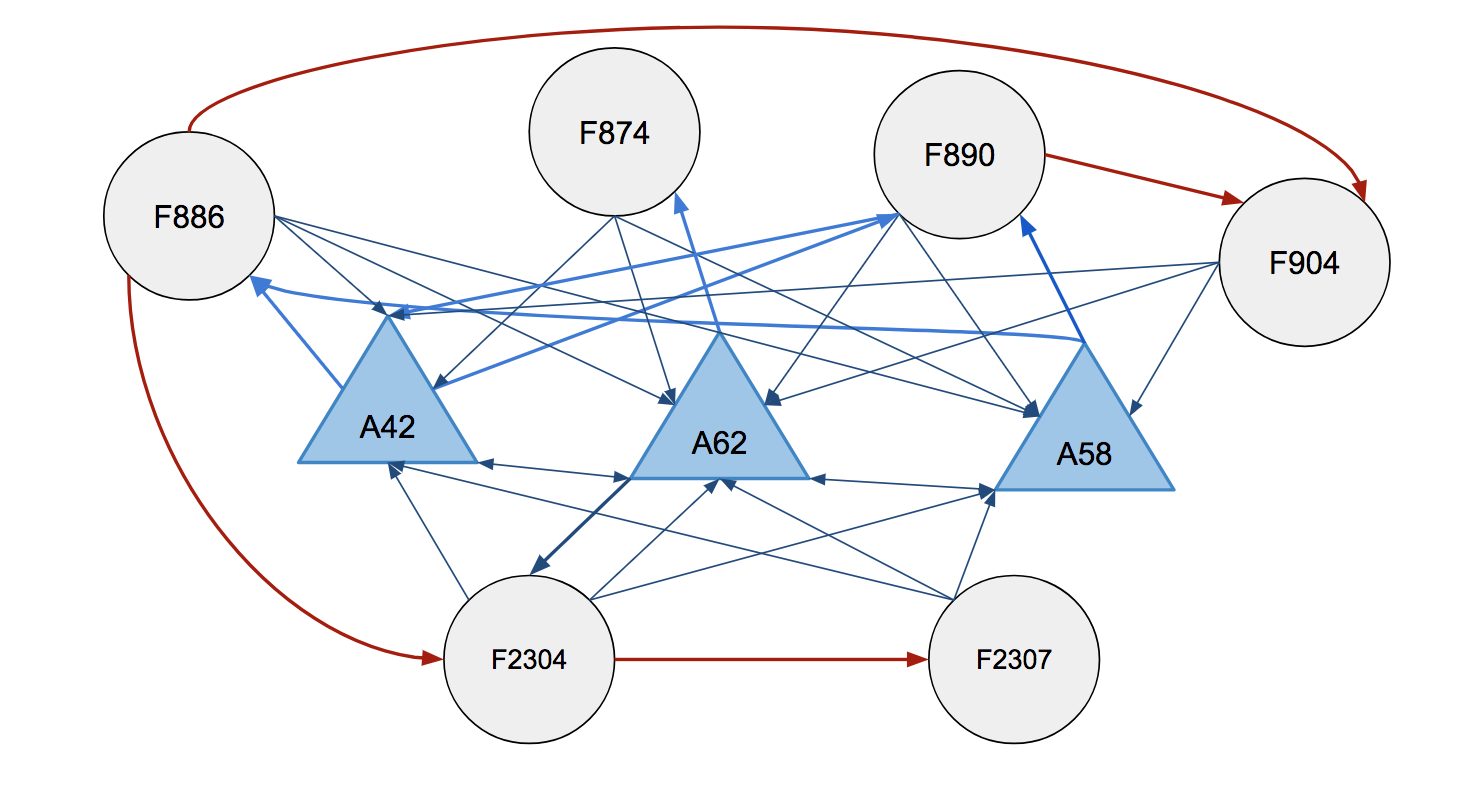
\includegraphics[width=15cm]{MasterThesis-master/updated-paths.png}\\
    \caption{Update feasible path after disruption}
    \label{fig:disruption}
\end{figure}

\begin{table}[h]
\renewcommand{\arraystretch}{1}
\begin{center}
\begin{tabular}{|c|c|c|c|c|c|c|c|c|c|}
\hline
\multicolumn{1}{|c|}{}
&\multicolumn{1}{|c|}{\(A42\)}
&\multicolumn{1}{c|}{\(A58\)}
&\multicolumn{1}{c|}{\(A62\)}
&\multicolumn{1}{|c|}{\(F866\)}
&\multicolumn{1}{c|}{\(F874\)}
&\multicolumn{1}{c|}{\(F890\)}
&\multicolumn{1}{c|}{\(F904\)}
&\multicolumn{1}{c|}{\(F2304\)}
&\multicolumn{1}{c|}{\(F2307\)}
\\  \hline
\(A42\) & 0 & 1 & 1 & 1 & 0 & 1 & 0 & 0 & 0
\\	\hline
\(A58\) & 1 & 0 & 1 & 1 & 0 & 1 & 0 & 0 & 0
\\	\hline
\(A62\) & 1 & 1 & 0 & 0 & 1 & 0 & 0 & 1 & 0
\\  \hline
\(F866\) & 1 & 1 & 1 & 0 & \textcolor{red}{0} & 0 & 1 & 1 & 0
\\	\hline
\(F874\) & 1 & 1 & 1 & 0 & 0 & 0 & 0 & 0 & 0
\\	\hline
\(F890\) & 1 & 1 & 1 & 0 & 0 & 0 & 1 & 1 & 0
\\  \hline
\(F904\) & 1 & 1 & 1 & 0 & 0 & 0 & 0 & 0 & 0
\\  \hline
\(F2304\) & 1 & 1 & 1 & 0 & 0 & 0 & 0 & 0 & 1
\\  \hline
\(F2307\) & 1 & 1 & 1 & 0 & 0 & 0 & 0 & 0 & 0
\\  \hline
\end{tabular}
\caption{Updated paths matrix}
\label{table:updated paths}
\end{center}
\end{table}

\section{Fitness calculation}\label{Fitness calculation}

 In this model, we use total cost as fitness, just same as the total distance in TSP. But when we get a completed path, a sequence list of aircraft and flights, how to transfer it into cost? We also use the example of Section\ref{Section:relationship} to explain.

Suppose that Fig.\ref{fig:one feasible solution} is one feasible solution. From this we can get a sequence list shown in Table.4.10.

\begin{figure}[h]
    \centering
    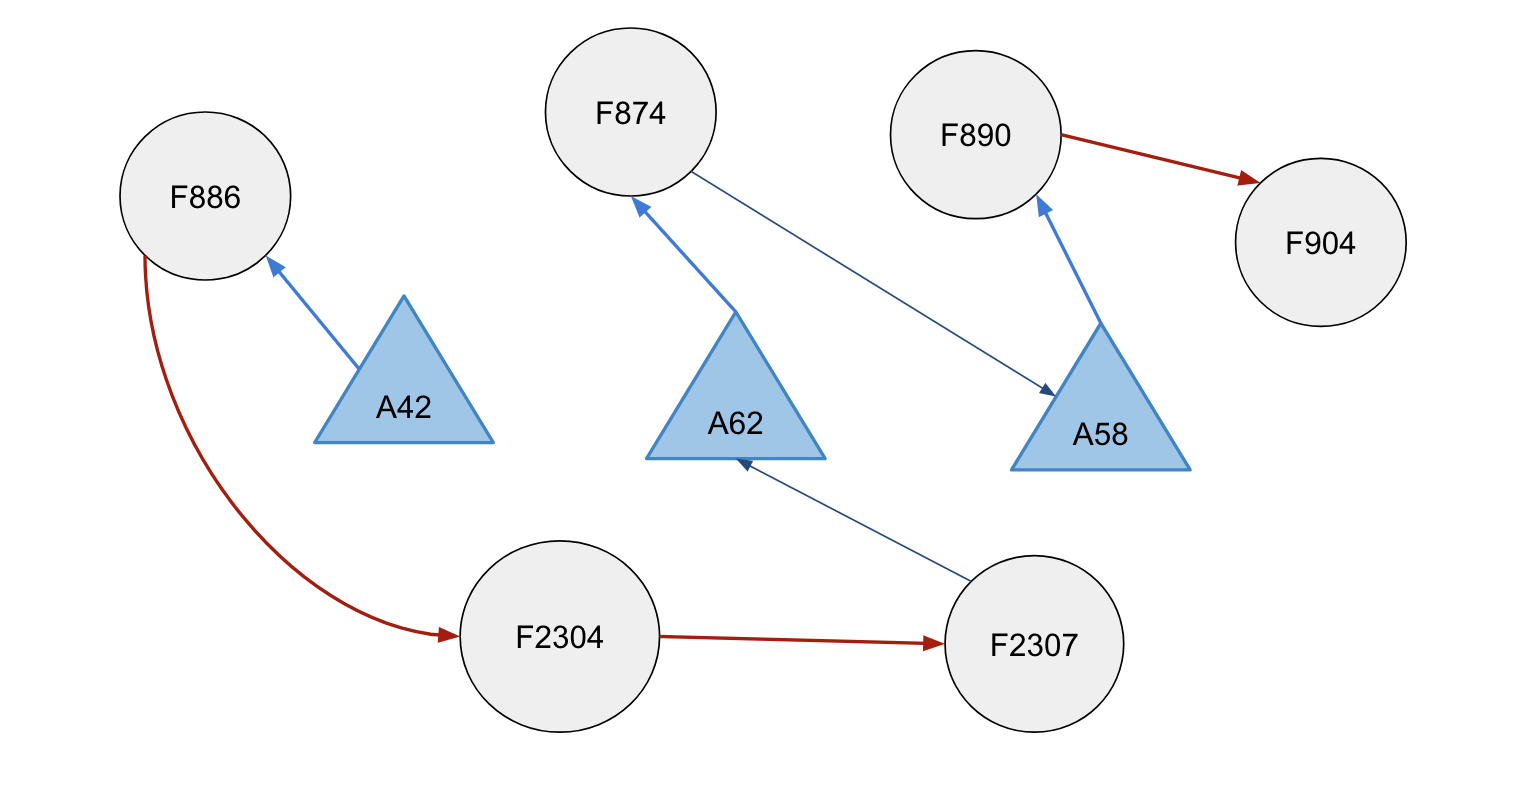
\includegraphics[width=15cm]{MasterThesis-master/feasible-solution1.png}\\
    \caption{One feasible solution}
    \label{fig:one feasible solution}
\end{figure}

\begin{table}[h]
\centering
\label{table: feasible solution}
\begin{tabular}{|c|c|c|c|c|c|c|c|c|}
\hline
A42 & F866 & F2304 & F2307 & A62 & F874 & A58 & F890 & F904 \\ \hline
\end{tabular}
\caption{Feasible Solution}
\end{table}

\begin{table}
\centering
\begin{tabular}{|l|l|l|l|l|l|l|l|l|} 
\hline
A42 & f866 & F874 & A62 & F2304 & F2307 & A58 & F890 & F904  \\
\hline
\end{tabular}
\caption{Original Schedule}
\label{table: Original schedule}
\end{table}



We can translate these two sequence list Table.4.10 and 4.11 into a easy-understanding way.
The feasible solution can be seen as:
\begin{itemize}
    \item \(A42\):  \(F866\), \(F2304\),\(2307\)
    \item \(A62\): \(F874\)
    \item \(A58\): \(F890\),\(F904\)
\end{itemize}
Also, the original schedule can be seen as:
\begin{itemize}
    \item \(A42\):  \(F866\), \(F874\)
    \item \(A62\): \(F2304\),\(2307\)
    \item \(A58\): \(F890\),\(F904\)
\end{itemize}
Above shows the pairs of aircraft and flights. Through the assignment pairs and we can get the actual departure time of each flight. Compare flights' status with original schedule, and use indicators mentioned in Section\ref{section:Objective function} to represent the status.
\begin{table}[h]
\renewcommand{\arraystretch}{1}
\begin{center}
\begin{tabular}{|c|c|c|c|}
\hline
\multicolumn{1}{|c|}{}
&\multicolumn{1}{c|}{\(x_f\)}
&\multicolumn{1}{c|}{\(y_f\)}
&\multicolumn{1}{c|}{\(z_f\)}
\\	\hline
\(F866\)  & 0 & 1 & 0
\\	\hline
\(F874\) & 1 & 0 & 0
\\	\hline
\(F890\) & 0 & 0 & 0 
\\  \hline
\(F904\) & 0 & 0 & 0
\\  \hline
\(F2304\) & 1 & 1 & 0
\\  \hline
\(F2307\) & 1 & 0 & 0
\\  \hline
\end{tabular}
\caption{Flight status}
\label{table:Flight status}
\end{center}
\end{table}

In Table\ref{table:Flight status}, \(x_f\) indicates if flight\(f\) is changed of aircraft, \(y_f\) indicates if flight\(f\) is delayed, \(z_f\) indicated if flight\(f\) is cancelled. And with these indicator combined with flight information in original schedule, we can calculate total cost applying Eq.\ref{func:total cost}, \ref{func:change aircraft cost}, \ref{func:delay cost}, \ref{func:cancel cost} and \ref{func:passsenger cost}.

\section{Ant Colony optimization implement}
When disruption break the original schedule, we intercept the flights suffered with break and aircraft still available then generate flight information dataset and aircraft status dataset. Using approach mentioned in last section, get feasible path matrix which involves value 0-1. 
Before start ant colony iteration, we need to generate a 
pheromone matrix which is an identity matrix.
At beginning, the first node that ant chooses must be the aircraft node. That means each route starts at an aircraft.

Ants choose the next node by the probability calculated by Eq.\ref{probability}. In this part, we will use both pheromone matrix and feasible path matrix.
The role of feasible path matrix is used as a heuristic factor. This matrix let probability of unfeasible path be 0 so that ants won't choose those path. And use feasible path matrix and pheromone matrix separately make it more easier to add modification on pheromone matrix. Changing pheromone globally will not influence the feasibility of paths.

After a group of ants all finish one iteration and create a completed route. We calculate the fitness which is the total cost in this model, and record the least one as well as the path of the least one. Then using reciprocal of this least fitness as change quantity:
\begin{equation}\label{func:delta pheromone}
    \Delta\rho = C * \left( \frac{1}{Total\_cost} \right)
\end{equation}
\(C\) is a constant to rationalize reciprocal of total cost because if $\frac{1}{Total\_cost}$ is too small, the pheromone matrix will be nearly no changed. Then we update pheromone matrix globally. 
\begin{equation}
    new\ \rho_k = max(1, \rho_k * (1-\mu) + \Delta\rho)
\end{equation}
Pheromone concentration should no less than original concentration 1. Because at a couple of iteration at beginning, the path is chosen randomly. So if some path is not be selected at first, their pheromone concentration still evaporate during iteration, then they will have less and less chance to be selected. So let the minimum value of pheromone concentration on each path can avoid this kind of problem.


\chapter{Experiment} \label{Experiment}

 In this section, we use real world data to test this proposed algorithm. The flight schedule dataset is from Chinese Xiamen Airline company. The dataset is over three days and there are total 2364 flights and 142 aircraft. We intercept the data on 5/6/2017, and select the disruption as an airport closure on 5/6/2017.
 
 On 5/6/2017, caused by typhoon, the  No.49 airport was closed:
 \begin{enumerate}
     \item restrict aircraft landing during 5/6/2017 14:00-5/720/17 17:00.
     \item restricts aircraft departure during 5/6/2017 16:00-5/7/2017 17:00. 
 \end{enumerate}
We only arrange flights on 5/6/2017, which has 341 flights despite those restricted by typhoon and 118 aircraft. We set parameter as below:
\begin{itemize}
    \item Ant population = 40
    \item Iteration times = 200
    \item evaporation rate = 0.15
\end{itemize}

With same parameter, we use both the method in this research and the method in \cite{sousa2015airline}. 
\begin{figure}[h]
    \centering
    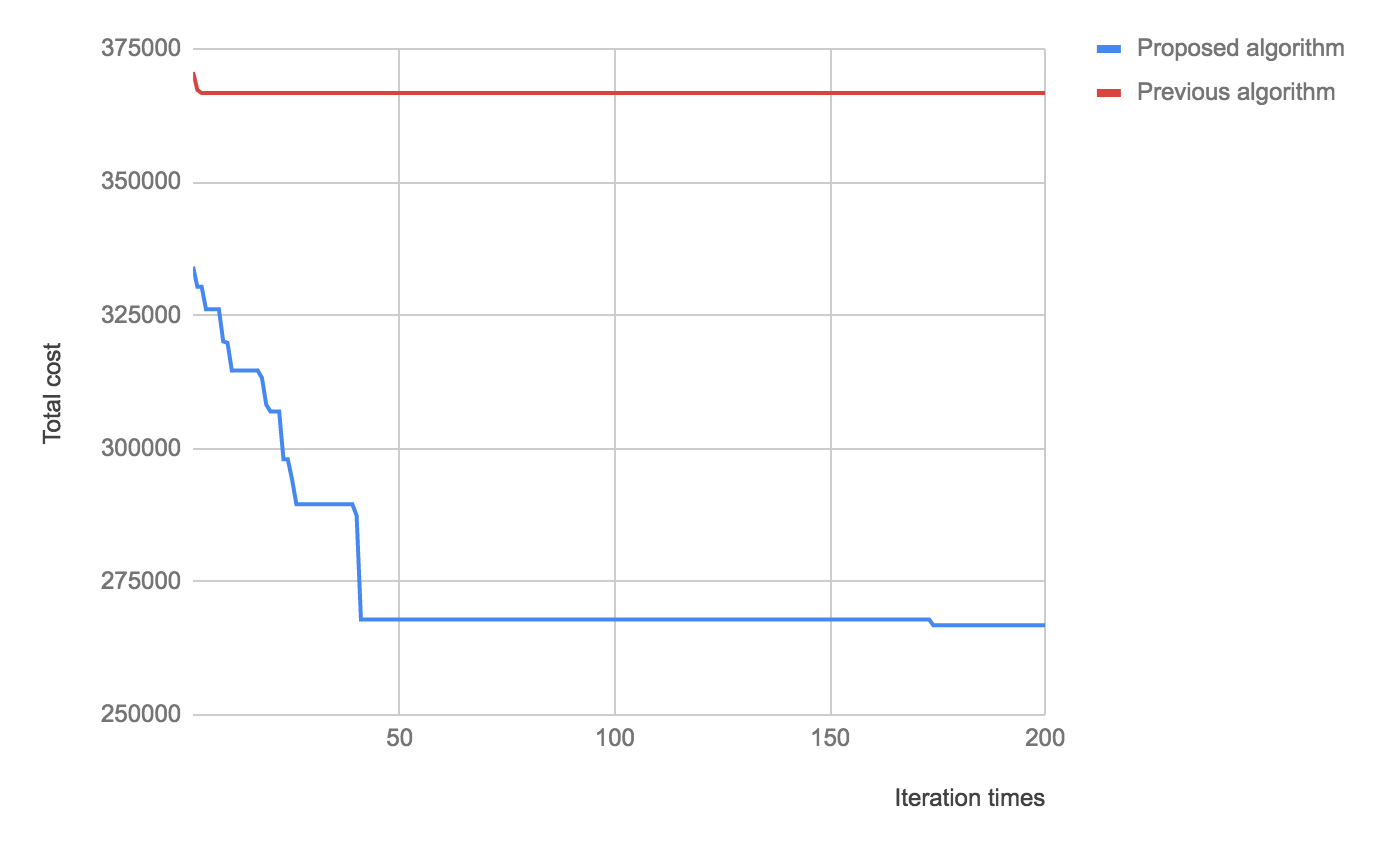
\includegraphics[width = 15cm]{MasterThesis-master/compare-two-algorithm.png}\\
    \caption{Compare two method}
    \label{fig:compare with past}
\end{figure}
In Fig.\ref{fig:compare with past}, we can see the using the method in \cite{sousa2015airline}, the algorithm converge too fast and rapidly fall in local optimum. And in our research, the result continues to decrease. So we can prove that adding randomness in selecting nodes part can make this model better and avoid to fall into local optimum too quickly.


\chapter{Conclusion and Future work} \label{Future work}

\section{Conclusion}
In this research, we apply ant colony optimization into flight schedule recovery problem. The main disruption we focus on is airport closure. And because this disruption always causes a large scale of influence on both flights and aircraft which makes it difficult for optimization, we develop rules to classify the affected flights and aircraft and make the data more tractable.

Based on past thesis\cite{sousa2015airline}, we build a model to make flight schedule suitable for ant colony optimization. Firstly we find out the relationship between flights and aircraft based original schedule and translate this relationship into feasible path web, then using this path web to implement ant colony optimization.

And for evaluation section, we use total cost to evaluate each solution. We divide the total cost into four parts, cost of changing aircraft pair, cost of delay, cost of cancellation and cost of maintaining passenger satisfaction. After one round of iteration, calculate the total cost and find the best one, then use the best one as changing quantity to make global update. 

Testing with real world dataset, this model shows it can output results in an acceptable time, and compared with the model of past research\cite{sousa2015airline}, it shows more randomness and can better optimization.

\section{Future Work}
In this research, although the results is continuously converge, but it still fall into local optimum after 100 times iteration. That causes many flights be cancelled. I think it should be add into more randomness.

Another disadvantage is now the calculating time is not efficient. It need to be improved in program structure and make the advantage more obviously compared with existing adjustment way.  


\bibliographystyle{IEEEtran}
\bibliography{LUOreference}


\end{document}
